% definit le type de document et ses options
\documentclass[a4paper,11pt]{article}

% des paquetages utiles classiques, en ajouter d'autres selon vos besoins
\usepackage[utf8]{inputenc}
\usepackage[T1]{fontenc}
\usepackage{amsmath}
\usepackage{amssymb,calc}
% \usepackage{fullpage}
% \usepackage{stmaryrd}
% \usepackage{url}
% \usepackage{xspace}
\usepackage[francais]{babel}

% Pour les figures
\usepackage{graphicx}

% Pour les listes à puces
\usepackage{enumitem}

\usepackage{indentfirst}

% Évite un conflit entre french babel et enumitem
\frenchbsetup{StandardLists=true}

\usepackage[standard,framed]{ntheorem}
\usepackage{framed}


\newcommand{\reff}[1]{(\ref{#1})}

\setlength{\parindent}{30pt}
\setlength{\parskip}{1ex}
\setlength{\textwidth}{15cm}
\setlength{\textheight}{24cm}
\setlength{\oddsidemargin}{0.2cm}
\setlength{\evensidemargin}{-.7cm}
\setlength{\topmargin}{-.5in}

% des commandes pratiques pour ecrire des maths :
\newcommand{\dx}{\,dx}
\newcommand{\dt}{\,dt}
\newcommand{\ito}{,\dotsc,}
\newcommand{\R}{\mathbb{R}}
\newcommand{\N}{\mathbb{N}}
\newcommand{\C}{\mathbb{C}}
\newcommand{\Z}{\mathbb{Z}}
\newcommand{\Poly}[1]{\mathcal{P}_{#1}}
\newcommand{\abs}[1]{\left\lvert#1\right\rvert}
\newcommand{\norm}[1]{\left\lVert#1\right\rVert}
\newcommand{\pars}[1]{\left(#1\right)}
\newcommand{\bigpars}[1]{\bigl(#1\bigr)}
\newcommand{\set}[1]{\left\{#1\right\}}

\DeclareMathOperator{\Sup}{Sup}
\DeclareMathOperator{\Max}{Max}

%
%\lstset{
%  literate=%
%  {À}{{\`A}}1 {Â}{{\^A}}1 {Ç}{{\c{C}}}1%
%  {à}{{\`a}}1 {â}{{\^a}}1 {ç}{{\c{c}}}1%
%  {É}{{\'E}}1 {È}{{\`E}}1 {Ê}{{\^E}}1 {Ë}{{\"E}}1% 
%  {é}{{\'e}}1 {è}{{\`e}}1 {ê}{{\^e}}1 {ë}{{\"e}}1%
%  {Ï}{{\"I}}1 {Î}{{\^I}}1 {Ô}{{\^O}}1%
%  {ï}{{\"i}}1 {î}{{\^i}}1 {ô}{{\^o}}1%
%  {Ù}{{\`U}}1 {Û}{{\^U}}1 {Ü}{{\"U}}1%
%  {ù}{{\`u}}1 {û}{{\^u}}1 {ü}{{\"u}}1%
%}

\newlength\dlf
\newcommand\alignedbox[2]{
  % #1 = before alignment
  % #2 = after alignment
    &
    \begingroup
    \settowidth\dlf{$\displaystyle #1$}
    \addtolength\dlf{\fboxsep+\fboxrule}
    \hspace{-\dlf}
    \boxed{#1 #2}
\endgroup
}

%%%%% PACKAGE AMSTHM :
% \newtheoremstyle{definition}
%   {20pt}   % ABOVESPACE
%   {20pt}   % BELOWSPACE
%   {}  % BODYFONT
%   {0pt}       % INDENT (empty value is the same as 0pt)
%   {\bfseries} % HEADFONT
%   {.}         % HEADPUNCT
%   {5pt plus 1pt minus 1pt} % HEADSPACE
%   {}          % CUSTOM-HEAD-SPEC

\newframedtheorem{ftheo}[theorem]{Theoreme}

\theoremstyle{plain} % default
\theorembodyfont{\normalfont}
\newframedtheorem{fdef}[definition]{Définition}

\renewtheorem{remark}{Remarque}

\newframedtheorem{coroll}{Corollaire}

\newtheorem{rappel}{Rappel}


\title{\huge \bfseries Méthodes itératives pour des systèmes linéaires}
\date{}


\begin{document}
\maketitle

On sait aujourd'hui résoudre numériquement des systèmes linéaires de l'ordre du million d'inconnues (et d'équations). Pour des \textbf{systèmes creux}, c'est-à-dire lorsque la matrice du système possède beaucoup de coefficients nuls, on arrive à une centaine de millions d'inconnues.
Les \textbf{systèmes pleins} font appel à des \textbf{méthodes directes}, qui donnent la solution exacte (aux erreurs d'arrondi près) en un nombre fini d'itérations, et seront décrites dans un chapitre ultérieur.

Pour les \textbf{très grands systèmes creux\footnote{Exemple : discrétisation par différences finies de problèmes aux limites pour des équations aux dérivées partielles ... + schéma}}
on utilise des \textbf{méthodes itératives}, où on construit une suite de vecteurs qui convergent vers la solution.

L'intérêt est que \textbf{ces méthodes ne manipulent pas la matrice}, mais seulement une fonction qui définit une suite par récurrence.

\begin{fdef}
    Soit $A \in M_n(\R)$ inversible et $b \in \R^n$. On appelle méthode itérative de résolution du système linéaire $Ax=b$, ($x \in \R^n$) 
    une méthode qui construit une suite récurrente $(x_k)_{k\geq0}$
    telle que $$(x_k \underset{k\to +\infty}{\longrightarrow} x) \Rightarrow Ax=b$$
    Une méthode itérative est convergente si $x_k \underset{k\to +\infty}{\longrightarrow}x$ pour toute condition initiale $x_0 \in \R^n$
\end{fdef}

\underline{Tests d'arrêt typiques :}

% Pour les listes à puces, met un point noir en Énum
\renewcommand{\labelitemi}{\textbullet}
\begin{itemize}
    \item $\frac{\|Ax_k - b \|}{\|b\|} < \varepsilon$ (norme du ``résidu'' / norme de b).

        Noter que : 
        \begin{align*} \frac{\|x_k-x\|}{\|x\|} 
            = \frac{\|A^{-1}(Ax_k-b)\|}{\|x\|} 
            & \leq \|A^{-1}\| \frac{\|b\|}{\|x\|}\varepsilon 
            \\ & \leq \|A^{-1}\| \|A\| \varepsilon, 
            \; \mbox{peut-être grand !}\end{align*}

\end{itemize}


Nous allons décrire ici des méthodes itératives avec ``splitting'' de A.


\section{Description générale :}

On considère ici le système
\begin{equation}
    \label{eq:eqdiff}
    Ax = b
\end{equation} 
où $A \in M_n(\R)$, $x \in \R^n$ et $b \in \R^n$. On suppose que la matrice $A$ est inversible.


On considère une décomposition de A (``splitting'') $A=M-N$ avec $M$ inversible et on considère l'itération :

\begin{equation}
\left\lbrace
\begin{array}{ccc}
    Mx_{k+1} & = & Nx_k + b\\
    \\
    x_0 \in \R^n
    \label{eq:2}
\end{array}\right.
\end{equation}

Si $x_k \to x$ quand $k \to +\infty$ alors $Mx = Nx + b$, càd $x$ est solution de \reff{eq:eqdiff}.

Le choix du splitting est très important pour la performance de la méthode :
\begin{itemize}
    \item Bien sûr la méthode doit être convergente (voir plus loin)
    \item On doit choisir $M$ de telle sorte que le système \reff{eq:2} soit beaucoup plus facile à résoudre que \reff{eq:eqdiff} (il faut résoudre \reff{eq:2} à chaque étape de l'itération).

        \underline{Exemples :} $M$ diagonale ou triangulaire, diagonale ou triangulaire par blocs.
\end{itemize}

Étudions les conditions de convergence de \reff{eq:2}.

\begin{fdef}
    Étant donné $A \in M_n(\C)$, on note $S_p(A)$ l'ensemble des valeurs propres de $A$ (ou ``spectre de A''). On appelle rayon spectral de $A$ et on note $\rho(A)$ :
\[
    \rho (A) = \underset{\lambda \in S_p(A)}{\Max|\lambda|}
\]
\end{fdef}

\begin{ftheo}
    La méthode \reff{eq:2} converge si et seulement si $$\rho(M^{-1}N) < 1$$
\end{ftheo}

La preuve complète de ce résultat sera étudiée en TD. Ici nous allons simplement montrer que $\rho(M^{-1}N)<1 \Rightarrow $ convergence de \reff{eq:2}, en admettant pour cela deux résultats.

\vspace{1cm}

\begin{ftheo}[de l'application contractante (dans $\R^n$) ]
    Soit $E$ un sous-ensemble de $\R^n$ fermé (et non vide). On considère une norme $\| \, \|$ sur $\R^n$.

    Soit $F : E \rightarrow E$ une application contractante, càd pour laquelle il existe $\alpha \in [0,1[$ tel que :
\[
    \| F(x) - F(y) \| \leq \alpha \| x-y \| \mbox{,} \: \: \forall x,y \in E
\]

    Alors il existe un unique $x^* \in E$ tel que $F(x^*)=x^*$ (càd $F$ admet un unique point fixe dans E). De plus, pour tout $x_0 \in E$, la suite définie par :
\[
    x_{k+1} = F(x_k)
\]
converge vers $x^*$, avec
\begin{equation}
    \| x^* - x_k \| \leq \frac{\alpha^k}{1 - \alpha} \| x_1 - x_0 \|
    \label{eq:3}
\end{equation}

Le système \reff{eq:2} s'écrit :

\begin{equation}
\left\lbrace
\begin{array}{c}
    \boxed{x_{k+1} = M^{-1}N x_k + M^{-1} b}\\
    \\
    x_0 \in \R^n
    \label{eq:5}
\end{array}\right.
\end{equation}

\end{ftheo}

\begin{remark}
   Théorème encore appelé ``Théorème du point fixe de Banach''. Le théorème reste vrai lorsque $E$ est un espace métrique complet.
\end{remark}

\begin{ftheo}[cf TD pour la démonstration]
    Soit $A \in M_n(\C)$ et $\varepsilon > 0$. Il existe une norme $\| \, \|$ sur $\C^n$ telle que :
\[
    \underbrace{\|A\|}_
    \text{\parbox[]{2cm}{norme sur $M_n(\C)$ induite par la norme $\| \, \|$ de $C^n$}}
        :=  \underset{\|x\|=1}{\Sup} \|Ax\| \leq \rho(A) + \varepsilon
\]
  
\end{ftheo}

Si $\rho (M^{-1}N) < 1$, il existe donc une norme matricielle induite telle que $\| M ^{-1} N \| \leq \rho (M^{-1} N) + \varepsilon < 1$. Alors :
\[
    \| F(x) - F(y) \| = \| M^{-1} N (x-y) \| \leq \underbrace{\| M^{^-1}N \|}_{< 1} \| x-y \|
\]

Donc $F : \R^n \rightarrow \R^n$ est une contraction.

Donc $\forall x_0 \in R^n$, la suite définie par \reff{eq:5} converge vers une limite $x \in \R^n$ unique, solution de $x = M^{-1}Nx+M^{-1}b$, c'est-à-dire $Ax=b$.

% Je ne sais pas comment présenter ces points
\vspace{1cm}
\underline{Vitesse de convergence :} Plus $\rho(M^{-1}N)$ est petit, plus $\|M^{-1}N\|$ peut être choisie petite et plus la convergence est rapide.
En effet, d'après \reff{eq:3} :
\[
    \|x-x_k\| \leq \frac{\|M^{-1}N\|^k}{1-\|M^{-1}N\|}\|x_1-x_0\|
\]

\vspace{1cm}
\underline{Exemple de splitting : } (peu utilisé)
\[
    M = \frac{1}{\alpha}I, \qquad N = \frac{1}{\alpha}I - A \qquad \Longrightarrow \qquad x_{k+1} = (I - \alpha A)x_k + \alpha b
\]
(méthode de Richardson stationnaire, ou du gradient à pas fixe)

Elle converge si et seulement si $\forall \lambda \in Sp(A), |1-\alpha \lambda | < 1$, c'est-à-dire toutes les valeurs propres de A se trouvent dans le disque (ouvert) de centre $(\frac{1}{\alpha}$ et rayon $\frac{1}{\alpha}$).

\section{Méthode de Jacobi}
On pose dans schéma \reff{eq:2} :
\[
    M = D \mbox{ avec $D$ diagonale et } d_{ii}=a_{ii}, \qquad N=D-A
\]

\begin{remark}
    Cela suppose $a_{ii} \ne 0 \; \forall i$ (si cette condition n'est pas vérifiée on peut permuter des lignes de $A$).
\end{remark}

\begin{ftheo}
    Si $A$ est à diagonale strictement dominante ($\rightarrow a_{ii}>0$ et $D$ inversible) alors la méthode de Jacobi converge.
\end{ftheo}

La démonstration sera vue en TD. On montre que le rayon spectral de la matrice $J = D^{-1}(D-A) = I - DA$ est $< 1$.

Nous avons rencontré ce type de matrices pour la discrétisation de problèmes aux limites dans le $1^{er}$ chapitre du cours.

\section{Méthodes de Gauss-Seidel et SOR}

On pose $A = D + L + U$ avec :

\[
   D =
   \begin{pmatrix}
       a_{00} & \cdots                      & 0      \\ 
       \vdots & a_{ii}\hspace{-0.5cm}\ddots & \vdots \\ 
       0      & \cdots                      & a_{nn}
   \end{pmatrix} 
   , L =
   \begin{pmatrix}
        0        & \cdots & 0      \\
        \vdots   & \ddots & \vdots \\
        a_{ij}(i>j)      & \cdots & 0
   \end{pmatrix}
   , U =
   \begin{pmatrix}
        0        & \cdots & a_{ij}(j>i)     \\
        \vdots   & \ddots & \vdots \\
        0        & \cdots & 0
   \end{pmatrix}
\]

Dans la méthode de Gauss-Seidel, on fixe :
\[
    M = D+L, \; N = -U
\]
La méthode s'écrit donc :
\[
    Dx_{k+1} = -Lx_{k+1}-Ux_k + b
\]
En notant $x_k = (x^{(k)}_1,\dots,x^{(k)}_n)$ on obtient pour $i=1..n$ :
\[
    a_{ii}x^{(k+1)}_i = - \sum_{j<i}a_{ij}x_j^{(k+1)} - \sum_{(j>i)}a_{ij}x_j^{(k)} + b_i
\]
Les méthodes de Jacobi et Gauss-Seidel ne sont guère utilisées. On leur préfère la méthode de relaxation.

La méthode SOR (``successive over-relaxation'', ou ``méthode de relaxation'', environ 1950) généralise Gauss-Seidel en introduisant un paramètre de relaxation $\omega \ne 0$,
que l'on ajuste afin d'accélérer la convergence de la méthode (avec un gain généralement très important si $\omega$ est bien choisi).

Pour $i=1,\dots,n$
\begin{equation}
\left\lbrace
\begin{array}{ccc}
    a_{ii}\tilde{x}_i^{(k+1)} & = & -\sum_{j<i} a_{ij}x_j^{(k+1)} - \sum_{j>i}a_{ij}x_j^{(k)} + b_i\\
    x_i^{(k+1)} & = & \omega \tilde{x_i}^{(k+1)} + (1-\omega)x_i^{(k)}
    \label{eq:4}
\end{array}\right.
\end{equation}
(Gauss-Seidel correspond à $\omega = 1$)

La méthode s'écrit (multiplier la seconde ligne par $a_{ii}$, et remplacer $a_{ii}\tilde{x_i}^{(k+1)}$ par son expression en fonction de $x_{k+1}$ et $x_k$)

\[
    Dx_{k+1}=(1-\omega)Dx_k - \omega L x_{k+1} - \omega U x_k + \omega b
\]

soit

\[
    (D + \omega L)x_{k+1} = [(1-\omega)D - \omega U]x_k + \omega b
\]

On a donc : 
\[
    M = \frac{1}{\omega}D + L, N = \frac{1-\omega}{\omega}D - U, M-N=D+L+U=A
\]

On note :
\[
    \mathcal{L}_{\omega} := (\frac{1}{\omega}D + L)^{-1}(\frac{1-\omega}{\omega}D - U)
\]
SOR converge si $\rho(\mathcal{L}_{\omega}<1$)

\begin{ftheo}[demo en TD]
    \begin{enumerate}
        \item
            Soit $A \in M_n(\R)$ inversible, avec $\forall i, a_{ii} \ne 0$
            Une condition nécessaire pour que SOR converge est que $\omega \in ]0,2[$.

        \item
            Si A est symétrique définie positive, alors $\forall \omega \in ]0,2[$, SOR converge 
    \end{enumerate}
\end{ftheo}

\begin{rappel}
    $A$ est symétrique définie positive si $A$ est symétrique, $^txAx = 0 \Rightarrow x = 0$, et $\forall x \in \R^n, {}^t\!xAx \geq 0$
\end{rappel}

\begin{coroll}
    Si $A$ est symétrique définie positive, alors la méthode de Gauss-Seidel converge.
    Nous avons rencontré ce type de matrices pour la discrétisation des problèmes aux limites dns le $1^{er}$ chapitre du cours (paragraphe 2), cas où la fonction $p$ est identiquement nulle.
\end{coroll}

\begin{remark}
    \begin{enumerate}
        \item Il y a des exemples où $A$ est symétrique définie positive et où la méthode de Jacobi n'est pas convergente.
        \item Si A est tridiagonale ($a_{ij}=0$ si $\abs{i-j}>1$) et $D$ inversible, on peut montrer que $\rho(\mathcal{L}_1)=\rho(J)^2$. Donc la méthode de Gauss-Seidel converge si et seulement si celle de Jacobi converge (et Gauss-Seidel converge plus vite).
        \item  Pour quelques types de matrices, on connaît la valeur de $\omega$ qui minimise $\rho (\mathcal{L}_{\omega})$.
            Pour $A$ tridiagonale (avec $D$ inversible), et si les valeurs propres de $J$ sont réelles, alors le paramètre de relaxation optimal dans SOR (c'est-à-dire la valeur de $\omega$ qui minimise $\rho (\mathcal{L}_{\omega})$) est > 1 (donc Gauss-Seidel ne donne pas la vitesse optimale de convergence).
        \item Pour optimiser empiriquement le choix de $\omega$ dans SOR, on peut évaluer le facteur de contractivité $\frac{\| x_{k+1} - x_k\|}{\| x_k - x_{k-1}\|}$ à partir du moment où $\|x_{k+1}-x_{k}\|$ décroît vers 0.
    \end{enumerate}
\end{remark}

\begin{figure}[]
    \centering
    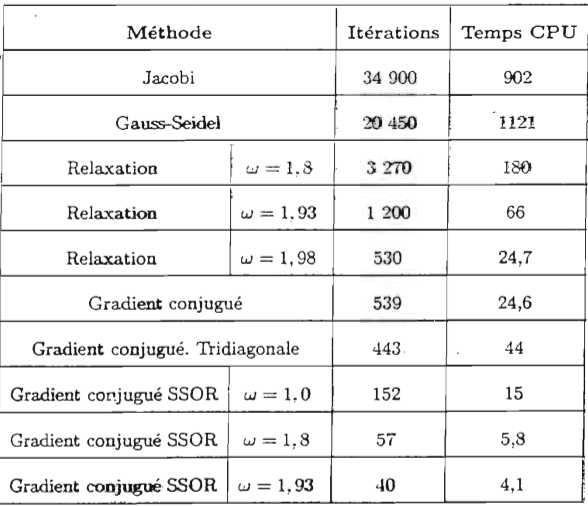
\includegraphics[scale=0.5]{tableau.png}
    \caption{Exemples pratiques}
    \label{fig:tableau}
\end{figure}

\end{document}



\end{document}




